\section{Luồng lưu lịch sử hội thoại}

Luồng này mô tả cách hệ thống lưu lại lịch sử trao đổi giữa người dùng và chatbot để phục vụ tra cứu lại cuộc hội thoại, thống kê, đánh giá chất lượng và làm giàu ngữ cảnh cho các xử lý tiếp theo. Đây là luồng dữ liệu hậu kỳ nhưng có giá trị lớn đối với cả trải nghiệm người dùng lẫn quản trị hệ thống.

\begin{figure}[H]
    \centering
    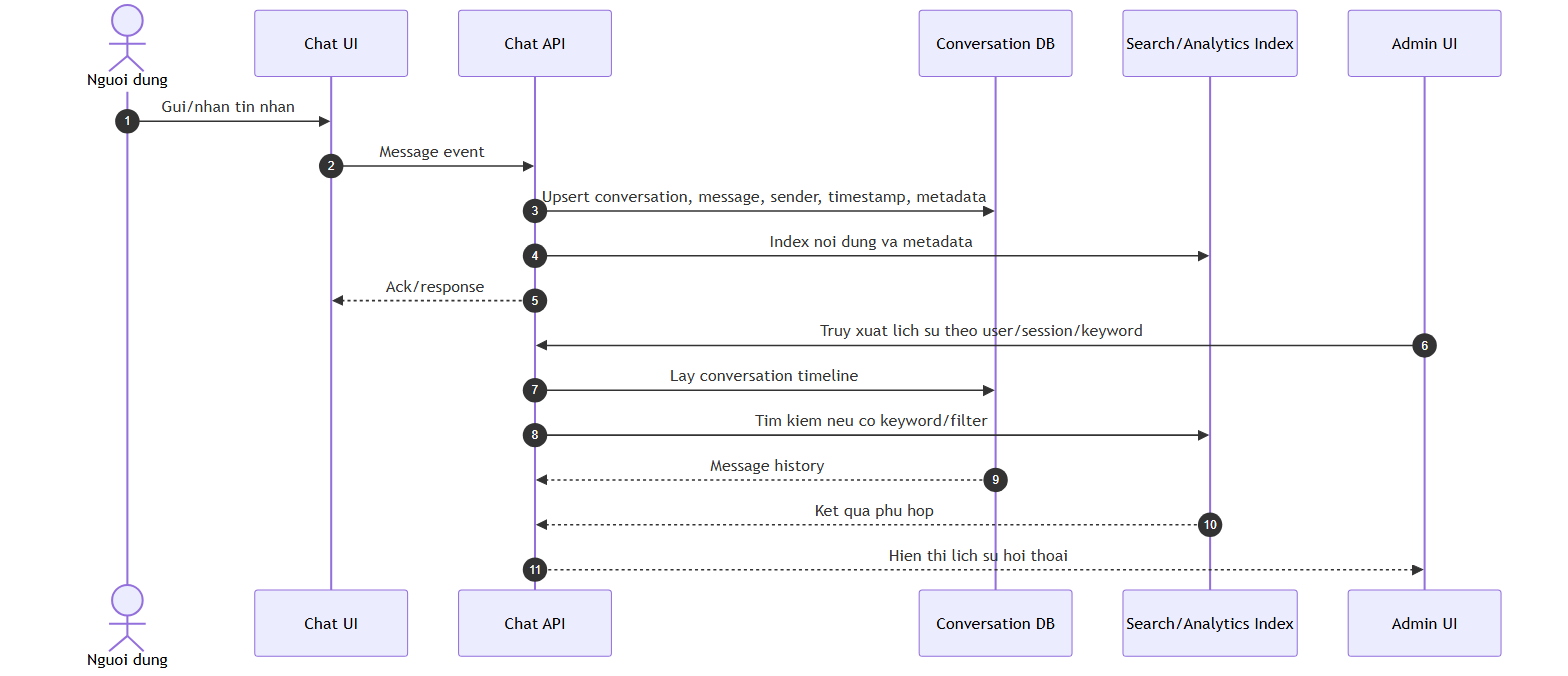
\includegraphics[width=\textwidth]{content/source/mermaid_sequence/seq_11.png}
    \caption{Luồng lưu lịch sử hội thoại}
\end{figure}

Theo sequence, sau khi người dùng gửi tin nhắn và chatbot trả phản hồi, backend ghép cặp các message thành một phần của phiên hội thoại và ghi chúng vào kho lưu trữ theo \path{conversationId}, \path{userId}, thời điểm tạo và cập nhật. Khi người dùng mở lại danh sách hội thoại hoặc xem chi tiết một cuộc trò chuyện, frontend gọi API lấy lịch sử để dựng lại toàn bộ ngữ cảnh đã có. Cơ chế này cũng giúp quản trị viên có dữ liệu để thống kê, kiểm thử hoặc truy nguyên khi xảy ra phản hồi bất thường.
